% Session 10 -- phase classification: where a local order parameter works and where it fails.
% Placement: sec. "Phase classification", after the Ising-gauge-theory paragraph.
% Rendered by figures/blender/s10f05_phaseclassification.py, labels in figures/overlays/s10f05_phaseclassification.tex.
\begin{aqmfigure}{fig:s10:phaseclass}{Why one phase-classification problem is easy and the other is
hard, seen from above with $\sigma=+1$ raised and $\sigma=-1$ sunk. \textbf{(a,b)} For the Ising
model (10.9) the magnetization of a single snapshot already separates the phases, and a network
trained on such snapshots only finds again the logic of a local order parameter of sessions 1, 5 and
6. \textbf{(c,d)} For the Ising gauge theory (10.10) the spins live on the \emph{bonds}, and the
$T=0$ condition $\prod_{i\in\partial p}\sigma_i = +1$ leaves an exponentially large degenerate
manifold. A typical ground state is random from bond to bond, so the magnetization is $\approx 0$ in
both columns and no quantity on a single bond can distinguish them. The difference is in the
four-spin structure of the plaquettes, which is marked by a cross where the product is $-1$, and the
convolutional network has to find by itself a function of the configuration that is sensitive to it.
The shaded star in (c) is a gauge flip of the four bonds at one vertex, which keeps every plaquette
product. This is the same obstruction that forced sessions 3 and 4 to go from local order parameters
to Chern numbers and Zak phases.}
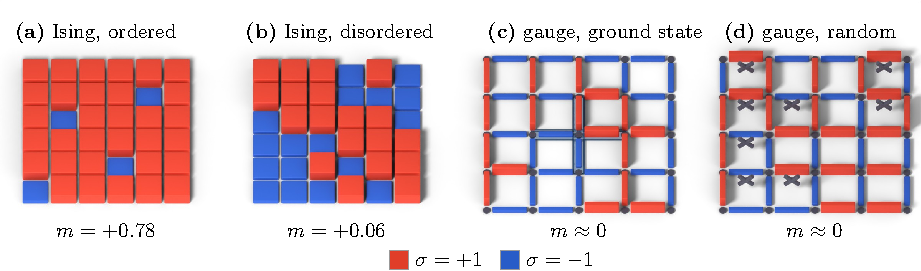
\includegraphics{figures/pdf/s10f05_phaseclassification.pdf}
\end{aqmfigure}
